\chapter{Polymères~: synthèse, structure et propriétés}\label{ch:b2:polymer-synthesis}

Les bas en nylon furent mis en vente en 1939. Ils sortaient d'un laboratoire qui s'était donné pour but,
quelques années plus tôt, de comprendre comment de petites molécules s'unissent en de longues, et qui
avait appris en chemin une leçon qui surprend tout chimiste la première fois~: pour un \omterm{def:b2:polymer-synthesis:polymer}{polymère} formé en
reliant des molécules bout à bout, un rendement de 99~\% ne suffit pas. Ce chapitre explique pourquoi,
décrit les deux façons dont les chaînes croissent, et relie la structure des chaînes aux propriétés des
matériaux.
% ledger: hist:nylon-production-1939

\begin{recall}
Le volume scolaire~: \omterm{def:b2:polymer-synthesis:polymer}{polymères}, \omterm{def:b2:polymer-synthesis:polymer}{monomères} et motifs, \omterm{def:b2:polymer-synthesis:polymer}{polymères} d'addition et de condensation,
thermoplastiques et thermodurcissables. Le volume de première année~: radicaux et homolyse,
carbocations et carbanions, approximation des états quasi stationnaires. \Cref{ch:b2:acyl-substitution}~:
esters et amides. \Cref{ch:b2:catalytic-cycles}~: insertion dans une liaison métal--carbone.
\end{recall}

\section{Les chaînes et leurs masses molaires}

\begin{definition}[Polymère]\label{def:b2:polymer-synthesis:polymer}
Un \emph{polymère}\index{polymere@polymère} est une substance formée de macromolécules, dont chacune est
construite par l'enchaînement répété de petites molécules, les \emph{monomères}\index{monomere@monomère}.
Le \emph{motif de répétition}\index{motif de repetition@motif de répétition}
est le plus petit groupe d'atomes dont la répétition constitue la chaîne~; le \emph{degré de
polymérisation}\index{degre de polymerisation@degré de polymérisation} $X$ d'une chaîne est le nombre
d'unités issues de monomères qu'elle contient.
\end{definition}

Un échantillon de \omterm{def:b2:polymer-synthesis:polymer}{polymère} synthétique n'est jamais formé de chaînes identiques~: c'est un mélange de
chaînes de longueurs différentes, et sa masse molaire est une moyenne, qui dépend de la façon dont on
compte les chaînes.

\begin{definition}[Masses molaires moyennes]\label{def:b2:polymer-synthesis:averages}
Pour un échantillon contenant $N_i$ chaînes de masse molaire $M_i$, la \emph{masse molaire moyenne en nombre}\index{masse molaire moyenne en nombre}
et la \emph{masse molaire moyenne en masse}\index{masse molaire moyenne en masse}
valent
\begin{equation*}
\bar M_n = \frac{\sum_i N_i M_i}{\sum_i N_i}, \qquad
\bar M_w = \frac{\sum_i N_i M_i^2}{\sum_i N_i M_i} = \sum_i w_i M_i,
\end{equation*}
où $w_i$ est la fraction massique des chaînes de masse $M_i$. La \emph{dispersité}\index{dispersite@dispersité}
$\text{\DH} = \bar M_w/\bar M_n$ vaut au moins 1, et ne vaut 1 que si toutes les chaînes ont la même
masse. Les moyennes $\bar X_n$ et $\bar X_w$ du \omterm{def:b2:polymer-synthesis:polymer}{degré de polymérisation} se définissent de la même
façon.
\end{definition}

La moyenne en nombre compte chaque chaîne une fois~; la moyenne en masse pondère chaque chaîne par sa
masse, si bien que les longues chaînes comptent davantage. Que $\text{\DH} \ge 1$ traduit l'inégalité $\left(\sum N_i M_i\right)^2 \le
\sum N_i \sum N_i M_i^2$ (Cauchy--Schwarz), avec égalité seulement si les $M_i$ sont égales.

\begin{method}[Calculer les moyennes]\label{met:b2:polymer-synthesis:averages}
\begin{enumerate}
  \item Traduire les données en quantités $N_i$ (ou nombres de chaînes) et masses $M_i$~; à partir des
        fractions massiques, $N_i \propto w_i/M_i$.
  \item $\bar M_n = \sum N_i M_i / \sum N_i$~; de façon équivalente, $1/\bar M_n = \sum w_i/M_i$.
  \item $\bar M_w = \sum w_i M_i$.
  \item $\text{\DH} = \bar M_w/\bar M_n$~; vérifier que $\bar M_w \ge \bar M_n$.
\end{enumerate}
\end{method}

\section{Croissance par étapes et croissance en chaîne}

\begin{definition}[Croissance par étapes et en chaîne]\label{def:b2:polymer-synthesis:step-chain}
Dans une \emph{polymérisation par étapes}\index{polymerisation par etapes@polymérisation par étapes}, deux
molécules quelconques portant des groupes fonctionnels complémentaires (\omterm{def:b2:polymer-synthesis:polymer}{monomères}, oligomères ou longues
chaînes) peuvent réagir, et les chaînes s'allongent en s'unissant les unes aux autres~: polyesters,
polyamides. Dans une \emph{polymérisation en chaîne}\index{polymerisation en chaine@polymérisation en chaîne},
un centre réactif (radical, ion ou liaison métal--carbone) ajoute des molécules de \omterm{def:b2:polymer-synthesis:polymer}{monomère} une à une à
l'extrémité d'une chaîne en croissance~: les \omterm{def:b2:polymer-synthesis:polymer}{polymères} des alcènes.
\end{definition}

\begin{method}[Par étapes ou en chaîne~?]\label{met:b2:polymer-synthesis:classify}
\begin{enumerate}
  \item Un \omterm{def:b2:polymer-synthesis:polymer}{monomère} portant deux groupes fonctionnels qui réagissent chacun avec le partenaire de l'autre
        (acide et alcool, acide et amine), souvent avec libération d'une petite molécule~: croissance par étapes.
  \item Un \omterm{def:b2:polymer-synthesis:polymer}{monomère} portant une double liaison \ce{C=C} (ou un cycle tendu) et un amorceur~: croissance en chaîne.
  \item Vérifier avec le déroulement de la réaction~: dans la croissance par étapes, le \omterm{def:b2:polymer-synthesis:polymer}{monomère} disparaît
        tôt et les longues chaînes n'apparaissent qu'à la toute fin~; dans la croissance en chaîne, des
        chaînes longues apparaissent dès le début tandis que le \omterm{def:b2:polymer-synthesis:polymer}{monomère} est consommé progressivement.
\end{enumerate}
\end{method}

\subsection*{Croissance par étapes}

Prenons un mélange équilibré de \omterm{def:b2:polymer-synthesis:polymer}{monomères} \ce{A-A} et \ce{B-B} (une diamine et un diacide), ou un
\omterm{def:b2:polymer-synthesis:polymer}{monomère} unique \ce{A-B}. Notons $p$ l'\emph{avancement}~: la fraction des groupes fonctionnels d'une
même sorte qui ont réagi.

\begin{theorem}[Équation de Carothers]\label{thm:b2:polymer-synthesis:carothers}
Dans une \omterm{def:b2:polymer-synthesis:step-chain}{polymérisation par étapes} de \omterm{def:b2:polymer-synthesis:polymer}{monomères} bifonctionnels exactement équilibrés, le \omterm{def:b2:polymer-synthesis:polymer}{degré de
polymérisation} moyen en nombre, compté en unités \omterm{def:b2:polymer-synthesis:polymer}{monomères}, vaut
\begin{equation*}
\bar X_n = \frac{1}{1 - p}.
\end{equation*}
\end{theorem}

\begin{proof}
Partons de $N_0$ molécules de \omterm{def:b2:polymer-synthesis:polymer}{monomère}, portant $N_0$ groupes \ce{A} et $N_0$ groupes \ce{B}. Chaque
réaction entre un \ce{A} et un \ce{B} unit deux molécules en une seule, et diminue donc d'une unité le
nombre de molécules. Après $pN_0$ réactions, il reste $N = N_0 - pN_0 = N_0(1-p)$ molécules qui se
partagent les $N_0$ unités \omterm{def:b2:polymer-synthesis:polymer}{monomères}~: $\bar X_n = N_0/N = 1/(1-p)$.
\end{proof}

\begin{corollary}[Déséquilibre]\label{cor:b2:polymer-synthesis:imbalance}
Si les groupes ne sont pas équilibrés, avec $r = N_{\ce{A}}/N_{\ce{B}} \le 1$ et $p$ l'avancement des
groupes minoritaires \ce{A},
\begin{equation*}
\bar X_n = \frac{1 + r}{1 + r - 2rp}, \qquad \text{au plus } \frac{1+r}{1-r} \text{ quand } p = 1.
\end{equation*}
\end{corollary}

\begin{proof}
Il y a au départ $(N_{\ce{A}} + N_{\ce{B}})/2$ molécules de \omterm{def:b2:polymer-synthesis:polymer}{monomère} bifonctionnel. Chaque molécule
linéaire possède deux extrémités de chaîne, chacune étant un groupe qui n'a pas réagi~; après réaction,
il reste $N_{\ce{A}}(1-p)$ groupes \ce{A} et $N_{\ce{B}} - pN_{\ce{A}}$ groupes \ce{B}, d'où $N = [N_{\ce{A}}(1-p) + N_{\ce{B}} -
pN_{\ce{A}}]/2$ molécules. En divisant, avec $N_{\ce{B}} = N_{\ce{A}}/r$~:
$\bar X_n = (1 + 1/r)/(1 - 2p + 1/r) = (1+r)/(1 + r - 2rp)$. Pour $r = 1$, on retrouve l'équation de Carothers.
\end{proof}

L'équation explique l'accroche du chapitre. Pour $p = 0.99$, soit un «~rendement de 99~\%~» de la réaction de liaison, $\bar X_n =
100$~; une fibre utile exige à peu près cette valeur ou davantage, si bien que la liaison doit dépasser
99~\%, avec des \omterm{def:b2:polymer-synthesis:polymer}{monomères} purs en quantités exactement égales et l'élimination de la petite molécule
libérée (eau, méthanol) pour continuer à déplacer l'équilibre. Un excès de 1~\% de l'un des \omterm{def:b2:polymer-synthesis:polymer}{monomères}
plafonne $\bar X_n$ à 201, même à \omterm{def:b2:continuous-reactors:conversion}{conversion} totale.

\begin{theorem}[Distribution de Flory]\label{thm:b2:polymer-synthesis:flory}
Dans une \omterm{def:b2:polymer-synthesis:step-chain}{polymérisation par étapes} d'avancement $p$, si chaque groupe a la même réactivité quelle que soit
la longueur de sa chaîne, la fraction en nombre et la fraction en masse des chaînes de $x$ unités valent
\begin{equation*}
n_x = (1-p)\,p^{\,x-1}, \qquad w_x = x(1-p)^2 p^{\,x-1},
\end{equation*}
et $\bar X_n = 1/(1-p)$, $\bar X_w = (1+p)/(1-p)$, de sorte que $\text{\DH} = 1 + p$, voisine de 2 à
\omterm{def:b2:continuous-reactors:conversion}{conversion} élevée.
\end{theorem}

\begin{proof}
Suivons une chaîne à partir d'une extrémité (un \omterm{def:b2:polymer-synthesis:polymer}{monomère} \ce{A-B}, pour simplifier). Chaque liaison le
long de la chaîne se forme avec la probabilité $p$, indépendamment des autres. La chaîne compte
exactement $x$ unités si les $x-1$ premières liaisons sont formées et la suivante non~: probabilité
$p^{\,x-1}(1-p)$, qui est $n_x$. Avec $\sum_{x\ge1} p^{\,x-1} =
1/(1-p)$ et ses dérivées $\sum x p^{\,x-1} = 1/(1-p)^2$ et $\sum x^2 p^{\,x-1} = (1+p)/(1-p)^3$~:
$\sum n_x = 1$, $\bar X_n = \sum x n_x = 1/(1-p)$, $w_x = x n_x/\bar X_n = x(1-p)^2p^{\,x-1}$, et
$\bar X_w = \sum x w_x = (1-p)^2(1+p)/(1-p)^3 = (1+p)/(1-p)$.
\end{proof}

\begin{omfigure}
\begin{tikzpicture}
\begin{axis}[width=0.46\linewidth, height=5cm, xmin=0, xmax=400, ymin=0,
  xlabel={degré de polymérisation $x$}, ylabel={fraction massique $w_x$}, label style={font=\small},
  tick label style={font=\scriptsize}, scaled y ticks=false,
  yticklabel style={/pgf/number format/fixed, /pgf/number format/precision=3},
  legend style={font=\scriptsize, at={(0.98,0.98)}, anchor=north east}, legend cell align=left]
\addplot[omDef, thick] table[x=x, y=p95] {figdata/out/bachelor-2-polymer-distributions-a.dat};
\addplot[omThm, thick] table[x=x, y=p98] {figdata/out/bachelor-2-polymer-distributions-a.dat};
\addplot[omMeth, thick] table[x=x, y=p99] {figdata/out/bachelor-2-polymer-distributions-a.dat};
\legend{$p = 0.95$, $p = 0.98$, $p = 0.99$}
\end{axis}
\end{tikzpicture}\hfill
\begin{tikzpicture}
\begin{axis}[width=0.46\linewidth, height=5cm, xmin=0, xmax=1, ymin=0, ymax=200,
  xlabel={avancement $p$}, ylabel={$\bar X_n$}, label style={font=\small},
  tick label style={font=\scriptsize}, xtick={0,0.2,0.4,0.6,0.8,1}]
\addplot[omDef, thick] table[x=p, y=Xn] {figdata/out/bachelor-2-polymer-distributions-b.dat};
\end{axis}
\end{tikzpicture}

{\small \omterm{def:b2:polymer-synthesis:step-chain}{Polymérisation par étapes} (modèles). À gauche~: distributions en masse de Flory
(\cref{thm:b2:polymer-synthesis:flory})~; le maximum se situe près de $\bar X_n$ et la distribution
s'élargit à mesure qu'il se déplace. À droite~: l'équation de Carothers~; $\bar X_n$ reste petit tant
que $p$ n'est pas très proche de 1.}
% figdata: bachelor-2/polymer-distributions.py parts a, b
\end{omfigure}

\subsection*{Croissance radicalaire en chaîne}

\begin{definition}[Étapes d'une polymérisation en chaîne]\label{def:b2:polymer-synthesis:chain-steps}
Une polymérisation radicalaire en chaîne comporte trois sortes d'étapes. Lors de l'\emph{amorçage}\index{amorcage@amorçage},
un \emph{amorceur radicalaire}\index{amorceur radicalaire} (une molécule à liaison faible, comme un
peroxyde ou un composé azoïque) se scinde par chauffage en radicaux, dont l'un s'additionne sur un
\omterm{def:b2:polymer-synthesis:polymer}{monomère}. Lors de la \emph{propagation}\index{propagation}, le radical en bout de chaîne additionne une
molécule de \omterm{def:b2:polymer-synthesis:polymer}{monomère} et reste un radical. Lors de la \emph{terminaison}\index{terminaison}, deux radicaux
se détruisent mutuellement, par combinaison (ils se lient) ou par dismutation (l'un arrache un atome
d'hydrogène à l'autre).
\end{definition}

\begin{omfigure}
\begin{align*}
&\text{amorçage~:} && \mathrm{I{-}I} \longrightarrow 2\,\mathrm{I^{\bullet}}, \qquad
\mathrm{I^{\bullet} + CH_2{=}CHPh \longrightarrow I{-}CH_2{-}\dot{C}HPh} \\
&\text{propagation~:} && {\sim}\mathrm{CH_2{-}\dot{C}HPh + CH_2{=}CHPh \longrightarrow}\;
{\sim}\mathrm{CH_2{-}CHPh{-}CH_2{-}\dot{C}HPh} \\
&\text{terminaison~:} && {\sim}\mathrm{CH_2{-}\dot{C}HPh + Ph\dot{C}H{-}CH_2}{\sim} \longrightarrow
{\sim}\mathrm{CH_2{-}CHPh{-}CHPh{-}CH_2}{\sim}
\end{align*}

{\small Polymérisation radicalaire du styrène. L'amorceur \ce{I-I} (le peroxyde de dibenzoyle, par
exemple) se scinde en deux radicaux~; chacun s'additionne sur l'extrémité \ce{CH2} du styrène, ce qui donne
le radical benzylique, plus stable~; la \omterm{def:b2:polymer-synthesis:chain-steps}{propagation} répète l'addition des milliers de fois~; deux radicaux
de chaîne se combinent et mettent fin aux deux chaînes. Le point marque l'électron célibataire.}
\end{omfigure}

\begin{theorem}[Vitesse de la polymérisation radicalaire]\label{thm:b2:polymer-synthesis:radical-rate}
Avec un amorceur qui se décompose avec la constante de vitesse $k_d$ et l'efficacité $f$ (la fraction
des radicaux qui amorcent une chaîne), une constante de \omterm{def:b2:polymer-synthesis:chain-steps}{propagation} $k_p$ et une constante de \omterm{def:b2:polymer-synthesis:chain-steps}{terminaison}
$k_t$ (vitesse de \omterm{def:b2:polymer-synthesis:chain-steps}{terminaison} $2k_t
[\mathrm{M^\bullet}]^2$), la vitesse de polymérisation en régime stationnaire vaut
\begin{equation*}
R_p = k_p [\mathrm M] \sqrt{\frac{f k_d [\mathrm I]}{k_t}}.
\end{equation*}
\end{theorem}

\begin{proof}
Soit $[\mathrm{M^\bullet}]$ la concentration totale des radicaux de chaîne, quelle que soit leur longueur.
Ils sont créés à la vitesse $R_i = 2fk_d[\mathrm I]$ (deux radicaux par molécule d'amorceur, dont une
fraction $f$ amorce des chaînes) et détruits à la vitesse $2k_t[\mathrm{M^\bullet}]^2$~; la \omterm{def:b2:polymer-synthesis:chain-steps}{propagation}
transforme un radical de chaîne en un autre et ne change pas leur nombre. L'approximation des états quasi
stationnaires appliquée à
$[\mathrm{M^\bullet}]$ donne $2fk_d[\mathrm I] = 2k_t[\mathrm{M^\bullet}]^2$, d'où $[\mathrm{M^\bullet}] =
\sqrt{fk_d[\mathrm I]/k_t}$. Le \omterm{def:b2:polymer-synthesis:polymer}{monomère} est consommé essentiellement par la \omterm{def:b2:polymer-synthesis:chain-steps}{propagation}, à $R_p =
k_p[\mathrm M][\mathrm{M^\bullet}]$.
\end{proof}

\begin{definition}[Longueur de chaîne cinétique]\label{def:b2:polymer-synthesis:chain-length}
La \emph{longueur de chaîne cinétique}\index{longueur de chaine cinetique@longueur de chaîne cinétique} $\nu$ est
le nombre moyen de molécules de \omterm{def:b2:polymer-synthesis:polymer}{monomère} additionnées par radical qui amorce une chaîne~: $\nu = R_p/R_i$.
\end{definition}

\begin{proposition}[Longueur de chaîne et amorceur]\label{prop:b2:polymer-synthesis:chain-length}
En régime stationnaire, $\nu = k_p[\mathrm M]/\bigl(2\sqrt{fk_dk_t[\mathrm I]}\bigr)$~: davantage d'amorceur
donne une polymérisation plus rapide mais des chaînes plus courtes. Avec une \omterm{def:b2:polymer-synthesis:chain-steps}{terminaison} par combinaison,
$\bar X_n = 2\nu$~; par dismutation, $\bar X_n = \nu$.
\end{proposition}

\begin{proof}
$\nu = R_p/R_i = k_p[\mathrm M]\sqrt{fk_d[\mathrm I]/k_t}/(2fk_d[\mathrm I]) =
k_p[\mathrm M]/\bigl(2\sqrt{fk_dk_t[\mathrm I]}\bigr)$. Chaque chaîne amorcée additionne en moyenne $\nu$
\omterm{def:b2:polymer-synthesis:polymer}{monomères}~; la combinaison unit deux de ces chaînes en une seule molécule, la dismutation en laisse deux.
\end{proof}

\begin{definition}[Polymérisation vivante]\label{def:b2:polymer-synthesis:living}
Une \emph{polymérisation vivante}\index{polymerisation vivante@polymérisation vivante} est une
\omterm{def:b2:polymer-synthesis:step-chain}{polymérisation en chaîne} sans \omterm{def:b2:polymer-synthesis:chain-steps}{terminaison} ni transfert~: toutes les chaînes démarrent ensemble et
continuent de croître tant qu'il reste du \omterm{def:b2:polymer-synthesis:polymer}{monomère}, et elles reprennent leur croissance quand on ajoute
du \omterm{def:b2:polymer-synthesis:polymer}{monomère}. La polymérisation anionique du styrène amorcée par le butyllithium dans un solvant aprotique
anhydre en est l'exemple classique.
\end{definition}

\begin{proposition}[Distributions étroites]\label{prop:b2:polymer-synthesis:living}
Dans une \omterm{def:b2:polymer-synthesis:living}{polymérisation vivante} où toutes les chaînes démarrent à la fois, le \omterm{def:b2:polymer-synthesis:polymer}{degré de polymérisation}
suit une loi de Poisson, et $\text{\DH} = 1 + \nu/(1+\nu)^2 \approx 1 + 1/\bar X_n$, où $\nu$ est le
nombre moyen de \omterm{def:b2:polymer-synthesis:polymer}{monomères} additionnés par chaîne.
\end{proposition}

\admitted

La distribution est celle du nombre d'additions, événements aléatoires indépendants de taux commun,
effectuées par chaque chaîne pendant la même durée~; la \omterm{def:b2:polymer-synthesis:averages}{dispersité} découle de la moyenne et de la variance
d'une loi de Poisson, toutes deux égales à $\nu$. Une chaîne vivante de 100 unités a donc $\text{\DH} \approx 1.01$,
contre près de 2 pour la même moyenne obtenue par croissance par étapes.

\begin{omfigure}
\begin{tikzpicture}
\begin{axis}[width=0.72\linewidth, height=5cm, xmin=0, xmax=150, ymin=0,
  xlabel={degré de polymérisation $x$}, ylabel={fraction massique $w_x$}, label style={font=\small},
  tick label style={font=\scriptsize}, scaled y ticks=false,
  yticklabel style={/pgf/number format/fixed, /pgf/number format/precision=3},
  legend style={font=\scriptsize, at={(0.98,0.98)}, anchor=north east}, legend cell align=left]
\addplot[omThm, thick] table[x=x, y=poisson] {figdata/out/bachelor-2-polymer-distributions-c.dat};
\addplot[omDef, thick] table[x=x, y=flory] {figdata/out/bachelor-2-polymer-distributions-c.dat};
\legend{vivante (Poisson), par étapes (Flory)}
\end{axis}
\end{tikzpicture}

{\small Deux échantillons de même $\bar X_n = 50$ (modèles). Les chaînes vivantes se pressent autour de 50 ($\text{\DH}
\approx 1.02$)~; les chaînes formées par étapes s'étalent du \omterm{def:b2:polymer-synthesis:polymer}{monomère} à plusieurs centaines d'unités ($\text{\DH} \approx
1.98$).}
% figdata: bachelor-2/polymer-distributions.py part c
\end{omfigure}

\begin{definition}[Copolymère]\label{def:b2:polymer-synthesis:copolymer}
Un \emph{copolymère}\index{copolymere@copolymère} est un \omterm{def:b2:polymer-synthesis:polymer}{polymère} construit à partir de deux \omterm{def:b2:polymer-synthesis:polymer}{monomères}
différents ou plus. Ses unités peuvent se succéder au hasard (copolymère statistique), en alternance, en
longues séquences de chacune (copolymère à blocs, préparé par \omterm{def:b2:polymer-synthesis:living}{polymérisation vivante}), ou sous forme de
chaînes latérales de l'un greffées sur un squelette de l'autre (copolymère greffé).
\end{definition}

\section{Structure des chaînes}

\begin{definition}[Tacticité]\label{def:b2:polymer-synthesis:tacticity}
Dans un \omterm{def:b2:polymer-synthesis:polymer}{polymère} vinylique \ce{-[CH2-CHR]_n-}, chaque carbone \ce{CHR} est un stéréocentre. La
\emph{tacticité}\index{tacticite@tacticité} décrit leurs configurations relatives le long de la chaîne
dessinée en zigzag plan~: dans une chaîne \emph{isotactique}\index{isotactique}, tous les groupes \ce{R}
sont du même côté du plan, dans une chaîne \emph{syndiotactique}\index{syndiotactique} ils alternent, et
dans une chaîne \emph{atactique}\index{atactique} ils sont disposés au hasard.
\end{definition}

\begin{omfigure}
\setchemfig{atom sep=1.5em}
\begin{tabular}{rl}
\small \omterm{def:b2:polymer-synthesis:tacticity}{isotactique} & \chemfig{[:-30]-[:30](<[:90])-[:-30]-[:30](<[:90])-[:-30]-[:30](<[:90])-[:-30]-[:30](<[:90])-[:-30]-[:30](<[:90])-[:-30]} \\[2pt]
\small \omterm{def:b2:polymer-synthesis:tacticity}{syndiotactique} & \chemfig{[:-30]-[:30](<[:90])-[:-30]-[:30](<:[:90])-[:-30]-[:30](<[:90])-[:-30]-[:30](<:[:90])-[:-30]-[:30](<[:90])-[:-30]} \\[2pt]
\small \omterm{def:b2:polymer-synthesis:tacticity}{atactique} & \chemfig{[:-30]-[:30](<[:90])-[:-30]-[:30](<[:90])-[:-30]-[:30](<:[:90])-[:-30]-[:30](<[:90])-[:-30]-[:30](<:[:90])-[:-30]}
\end{tabular}
\par\vspace{6pt}

{\small Le polypropène dessiné en zigzag dans le plan de la page~; chaque groupe méthyle est un coin plein
(vers le lecteur) ou un coin hachuré (en arrière). \omterm{def:b2:polymer-synthesis:tacticity}{Isotactique}~: tous les méthyles d'un même côté~;
\omterm{def:b2:polymer-synthesis:tacticity}{syndiotactique}~: en alternance~; \omterm{def:b2:polymer-synthesis:tacticity}{atactique}~: irrégulier.}
\end{omfigure}

Des chaînes régulières peuvent s'empiler côte à côte en régions cristallines~; des chaînes irrégulières
ne le peuvent pas. Le polypropène \omterm{def:b2:polymer-synthesis:tacticity}{isotactique}, préparé avec les catalyseurs métalliques du volume de
troisième année, est en partie cristallin, dur et à haut point de fusion~; le polypropène \omterm{def:b2:polymer-synthesis:tacticity}{atactique} est
un matériau amorphe, mou et collant. Un \omterm{def:b2:polymer-synthesis:polymer}{polymère} est rarement entièrement cristallin~: des cristallites
sont noyées dans des régions amorphes où les chaînes sont enchevêtrées.

\begin{definition}[Transitions thermiques]\label{def:b2:polymer-synthesis:transitions}
Le \emph{taux de cristallinité}\index{taux de cristallinite@taux de cristallinité} d'un \omterm{def:b2:polymer-synthesis:polymer}{polymère} est la
fraction massique de celui-ci qui se trouve dans des régions cristallines. La \emph{température de
transition vitreuse}\index{temperature de transition vitreuse@température de transition vitreuse}
$T_g$ est la température au-dessous de laquelle les régions amorphes forment un verre rigide, leurs
segments de chaîne étant incapables de bouger, et au-dessus de laquelle elles deviennent caoutchouteuses~;
les régions cristallines fondent à une température plus élevée, $T_m$.
\end{definition}

Le polystyrène et le poly(méthacrylate de méthyle) sont amorphes, avec une $T_g$ supérieure à la
température ambiante~: ce sont des verres rigides et transparents. Le caoutchouc naturel a une $T_g$
bien inférieure à la température ambiante. Le polyéthène, de $T_g$ très inférieure à la température
ambiante mais fortement cristallin, est résistant et souple~: ses cristallites maintiennent ensemble les
parties amorphes caoutchouteuses.

\begin{omfigure}
\begin{tikzpicture}[x=1cm, y=1cm]
\draw[->] (0,0) -- (8.6,0) node[below left, font=\small] {température};
\draw[->] (0,0) -- (0,4.6) node[above, font=\small] {$\log$ module};
\draw[omDef, very thick] (0.2,4) .. controls (1.8,3.95) and (2.4,3.9) .. (2.8,3.6)
  .. controls (3.3,3.0) and (3.4,1.9) .. (4.0,1.75) -- (6.0,1.6)
  .. controls (6.7,1.5) and (7.0,0.8) .. (7.8,0.35);
\draw[omThm, very thick, dashed] (4.0,1.75) -- (6.0,1.7) .. controls (6.6,1.68) and (7.2,1.65) .. (8.2,1.6);
\draw[densely dotted] (3.2,0) node[below, font=\small] {$T_g$} -- (3.2,4.2);
\node[font=\footnotesize, align=center] at (1.4,3.4) {vitreux};
\node[font=\footnotesize, align=center] at (4.0,3.3) {transition};
\node[font=\footnotesize, align=center] at (5.0,2.3) {plateau élastique};
\node[font=\footnotesize, align=center, omDef] at (7.6,1.15) {s'écoule};
\node[font=\footnotesize, align=center, omThm] at (7.7,2.0) {réticulé};
\end{tikzpicture}
\par\vspace{4pt}

{\small Module (rigidité) d'un \omterm{def:b2:polymer-synthesis:polymer}{polymère} amorphe en fonction de la température, schématique. Au-dessous de
$T_g$, le matériau est un verre~; dans la transition, le module chute de plusieurs ordres de grandeur~;
sur le plateau élastique, les chaînes enchevêtrées se comportent comme un caoutchouc~; à plus haute
température, un \omterm{def:b2:polymer-synthesis:polymer}{polymère} linéaire s'écoule (trait plein), tandis qu'un \omterm{def:b2:polymer-synthesis:polymer}{polymère} réticulé conserve son
plateau jusqu'à sa décomposition (tirets).}
\end{omfigure}

\section{Propriétés et usages}

\begin{definition}[Élastomère]\label{def:b2:polymer-synthesis:elastomer}
Un \emph{élastomère}\index{elastomere@élastomère} est un \omterm{def:b2:polymer-synthesis:polymer}{polymère} utilisé au-dessus de sa \omterm{def:b2:polymer-synthesis:transitions}{température de
transition vitreuse}, dont les chaînes sont faiblement réticulées~: il peut être étiré jusqu'à plusieurs
fois sa longueur et reprend sa forme quand on le relâche.
\end{definition}

Les quatre grandes classes de matériaux \omterm{def:b2:polymer-synthesis:polymer}{polymères} découlent de la structure et des transitions. Les
thermoplastiques, linéaires ou ramifiés, vitreux ou semi-cristallins à température ambiante, se
ramollissent à la chaleur et peuvent être moulés encore et encore~: polyéthène, polypropène, polystyrène,
PET. Les \omterm{def:b2:polymer-synthesis:elastomer}{élastomères} sont des chaînes faiblement réticulées au-dessus de leur $T_g$~: le caoutchouc
vulcanisé, dans lequel des ponts soufrés relient les chaînes. Les fibres sont des chaînes alignées par
étirage, avec de fortes interactions entre elles~: les liaisons hydrogène entre les groupes amide du
nylon. Les thermodurcissables sont des réseaux densément réticulés formés pendant le moulage~: les résines
époxy et phénol--formaldéhyde, qu'on ne peut pas refondre. Seuls les thermoplastiques se recyclent par
fusion~; le volume scolaire a donné l'ampleur du problème.

\begin{omfigure}
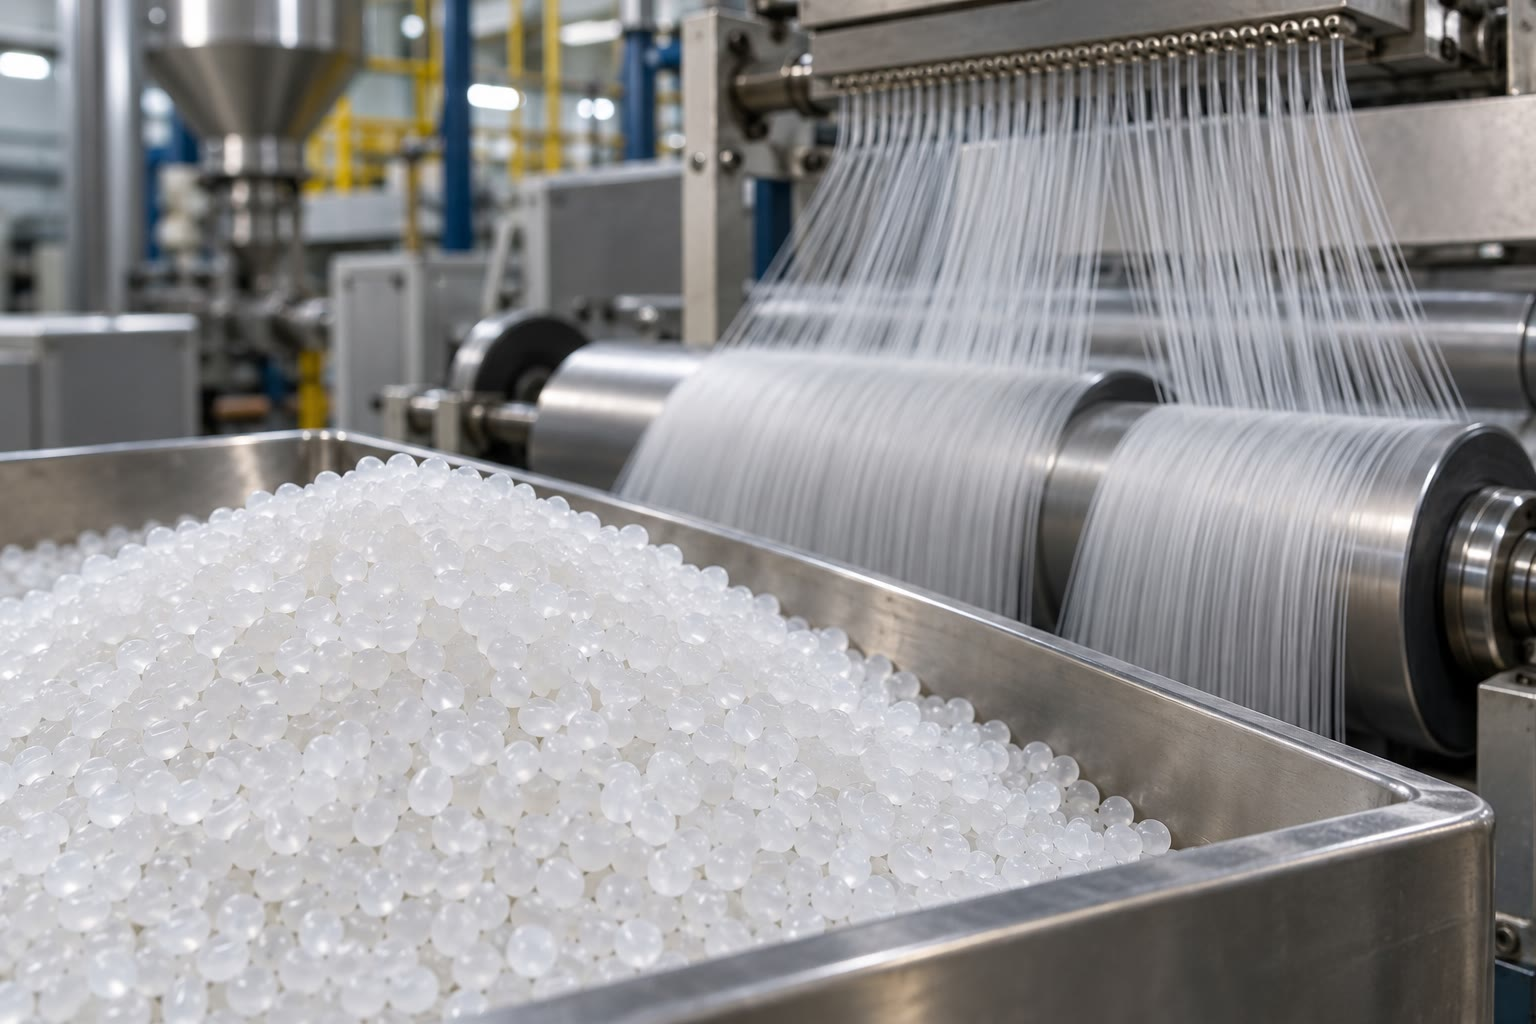
\includegraphics[width=0.58\linewidth]{images/book3/ai/b2-29-pellets.jpg}

{\small Granulés de \omterm{def:b2:polymer-synthesis:polymer}{polymère} dans une usine, forme sous laquelle les thermoplastiques sont vendus, et
fibres étirées à la sortie d'une filière sur des rouleaux tournants à l'arrière-plan (illustration).}
\end{omfigure}

\begin{history}[Un rendement de 99~\% ne suffit pas]
\begin{minipage}[t]{0.2\linewidth}
\vspace{0pt}
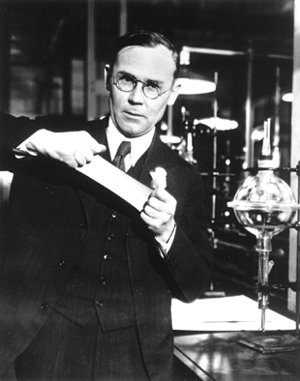
\includegraphics[width=\linewidth]{images/book3/carothers.jpg}
\end{minipage}\hfill
\begin{minipage}[t]{0.76\linewidth}
\vspace{0pt}
Wallace Carothers, jeune enseignant d'université recruté par un laboratoire industriel pour y faire de
la recherche fondamentale, construisit de longues molécules à partir de réactions bien connues, et ses
résultats appuyèrent fortement l'idée, alors contestée, que les \omterm{def:b2:polymer-synthesis:polymer}{polymères} sont des molécules ordinaires,
seulement très longues. Son équipe prépara des polyesters, puis, à partir de 1934, des polyamides~;
l'équation qui porte son nom explique pourquoi seules des \omterm{def:b2:continuous-reactors:conversion}{conversions} extrêmes donnaient des fibres. Le
nylon fut produit à partir de 1939. (Photographie~: photographe inconnu, domaine public~; Wikimedia Commons.)
% ledger: hist:polyamides-1934, hist:nylon-production-1939
\end{minipage}
\end{history}

\begin{safety}{\ghs[5mm]{GHS01}\,\ghs[5mm]{GHS02}\,\ghs[5mm]{GHS05}\,\ghs[5mm]{GHS07}\,\ghs[5mm]{GHS08}\,\ghs[5mm]{GHS09}}
Le styrène est inflammable et dangereux pour la santé. Le peroxyde de dibenzoyle est un oxydant
explosif à l'état sec et se conserve humide et au frais. L'hexane-1,6-diamine et l'acide hexanedioïque
sont corrosifs pour les yeux.
% ledger: ghs:styrene, ghs:BPO, ghs:hexanediamine, ghs:adipic-acid
\end{safety}

\section{Exercices}

\begin{exercise}[$\star$]\label{exo:b2:polymer-synthesis:1}
Représenter les \omterm{def:b2:polymer-synthesis:polymer}{motifs de répétition} du polyéthène, du polypropène, du poly(chlorure de vinyle), du polystyrène et du nylon-6,6.
\end{exercise}

\begin{exercise}[$\star$]\label{exo:b2:polymer-synthesis:2}
Croissance par étapes ou en chaîne~: le PET à partir de l'éthane-1,2-diol et de l'acide
benzène-1,4-dicarboxylique~; le polystyrène~; le nylon-6,6~; le poly(méthacrylate de méthyle)~;
l'acide polylactique à partir de l'acide 2-hydroxypropanoïque~?
\end{exercise}

\begin{exercise}[$\star$]\label{exo:b2:polymer-synthesis:3}
Un polystyrène a $\bar X_n = 1000$. Calculer $\bar M_n$, en négligeant les groupes terminaux.
\end{exercise}

\begin{exercise}[$\star$]\label{exo:b2:polymer-synthesis:4}
Une chaîne de polypropène dessinée en zigzag plan porte ses groupes méthyle du côté du lecteur, puis en
arrière, puis vers le lecteur, puis en arrière, et ainsi de suite. Nommer sa \omterm{def:b2:polymer-synthesis:tacticity}{tacticité}. Pourrait-elle cristalliser~?
\end{exercise}

\begin{exercise}[$\star\star$]\label{exo:b2:polymer-synthesis:5}
Un échantillon est un mélange de masses égales de deux fractions, de masses molaires \qty{10}{kg/mol} et
\qty{100}{kg/mol}. Calculer $\bar M_n$, $\bar M_w$ et la \omterm{def:b2:polymer-synthesis:averages}{dispersité}.
\end{exercise}

\begin{exercise}[$\star\star$]\label{exo:b2:polymer-synthesis:6}
Calculer $\bar X_n$ pour une \omterm{def:b2:polymer-synthesis:step-chain}{polymérisation par étapes} équilibrée à $p = 0.98$ et à $p = 0.995$.
\end{exercise}

\begin{exercise}[$\star\star$]\label{exo:b2:polymer-synthesis:7}
On mélange un diacide et une diamine avec un excès de 1~\% (en moles) de diamine. Quelle est la plus grande
valeur de $\bar X_n$ que l'on peut atteindre~?
\end{exercise}

\begin{exercise}[$\star\star$]\label{exo:b2:polymer-synthesis:8}
Dans une polymérisation radicalaire, on double la concentration en amorceur. Par quel facteur la vitesse
de polymérisation et la \omterm{def:b2:polymer-synthesis:chain-length}{longueur de chaîne cinétique} sont-elles multipliées~?
\end{exercise}

\begin{exercise}[$\star\star$]\label{exo:b2:polymer-synthesis:9}
Le poly(chlorure de vinyle) est rigide~; les tuyaux d'arrosage qui en sont faits sont souples parce qu'ils
contiennent un plastifiant, petite molécule glissée entre les chaînes. Expliquer à l'aide de la transition vitreuse.
\end{exercise}

\begin{exercise}[$\star\star\star$]\label{exo:b2:polymer-synthesis:10}
Montrer que la distribution en masse de Flory $w_x = x(1-p)^2p^{\,x-1}$, vue comme une fonction de la
variable continue $x$, est maximale en $x = -1/\ln p$, et que cette valeur est voisine de $\bar X_n$ quand $p$ est voisin de 1.
\end{exercise}

\begin{exercise}[$\star\star\star$]\label{exo:b2:polymer-synthesis:11}
Le PET est préparé en deux temps~: le benzène-1,4-dicarboxylate de diméthyle avec un excès
d'éthane-1,2-diol donne le benzène-1,4-dicarboxylate de bis(2-hydroxyéthyle) et du méthanol~; ce diester
est ensuite chauffé sous vide et polymérise en libérant de l'éthane-1,2-diol. Écrire les deux étapes et
expliquer comment la seconde résout le problème de stœchiométrie posé par l'équation de Carothers.
\end{exercise}

\begin{exercise}[$\star\star\star$]\label{exo:b2:polymer-synthesis:12}
Dans une copolymérisation radicalaire des \omterm{def:b2:polymer-synthesis:polymer}{monomères} 1 et 2, la composition instantanée du \omterm{def:b2:polymer-synthesis:copolymer}{copolymère} est
donnée par $\dfrac{\mathrm d[\mathrm M_1]}{\mathrm d[\mathrm M_2]} = \dfrac{[\mathrm M_1](r_1[\mathrm M_1]
+ [\mathrm M_2])}{[\mathrm M_2]([\mathrm M_1] + r_2[\mathrm M_2])}$, où $r_1$ et $r_2$ sont les
rapports de réactivité (données de l'exercice~: $r_1 = 2.0$, $r_2 = 0.5$). Calculer le rapport des unités
dans le \omterm{def:b2:polymer-synthesis:copolymer}{copolymère} formé à partir d'une alimentation équimolaire. Que se passe-t-il si $r_1 = r_2 = 0$~?
\end{exercise}

\section{Problème~: du nylon-6,6 au kilogramme}

\begin{problem}[{Problème du week-end --- les monomères et le sel de nylon, l'équation de Carothers, un
déséquilibre délibéré, la distribution de Flory et l'eau libérée}]
\label{pb:b2:polymer-synthesis:1}
Le nylon-6,6 est préparé à partir de l'hexane-1,6-diamine et de l'acide hexanedioïque. Les groupes
terminaux sont négligés partout. Masses molaires (\unit{g/mol})~: C 12.011, H 1.008, N 14.007, O 15.999.
% ledger: aw:C, aw:H, aw:N, aw:O, ghs:hexanediamine, ghs:adipic-acid

\medskip
\noindent\textbf{Partie I --- \omterm{def:b2:polymer-synthesis:polymer}{Monomères} et \omterm{def:b2:polymer-synthesis:polymer}{motif de répétition}.}
\begin{enumerate}
  \item Écrire les formules des deux \omterm{def:b2:polymer-synthesis:polymer}{monomères}.
  \item Écrire l'équation de formation d'une liaison amide.
  \item Les \omterm{def:b2:polymer-synthesis:polymer}{monomères} sont d'abord associés en un sel 1\,:\,1, cristallisé dans une solution. Pourquoi~?
  \item Donner le \omterm{def:b2:polymer-synthesis:polymer}{motif de répétition} du nylon-6,6, sa formule et sa masse molaire.
  \item Quelle est la masse molaire moyenne $M_0$ d'une unité de la chaîne issue d'un \omterm{def:b2:polymer-synthesis:polymer}{monomère}~?
  \item Que comptent les deux nombres du nom «~6,6~»~?
\end{enumerate}

\medskip
\noindent\textbf{Partie II --- L'équation de Carothers.}
\begin{enumerate}[resume]
  \item Calculer $\bar X_n$ et $\bar M_n$ à $p = 0.98$.
  \item Même question à $p = 0.99$.
  \item Expliquer la remarque «~un rendement de 99~\% ne suffit pas~».
  \item Quel avancement donne $\bar M_n = \qty{10}{kg/mol}$~?
  \item Comment pousse-t-on l'avancement aussi haut en pratique~?
  \item Pourquoi les \omterm{def:b2:polymer-synthesis:polymer}{monomères} doivent-ils être très purs~?
\end{enumerate}

\medskip
\noindent\textbf{Partie III --- Un déséquilibre délibéré.}
\begin{enumerate}[resume]
  \item La diamine est utilisée avec un excès molaire de 1~\%. Calculer $r$.
  \item Calculer les plus grandes valeurs de $\bar X_n$ et de $\bar M_n$ que l'on peut alors atteindre.
  \item Calculer $\bar X_n$ à $p = 0.99$ avec ce déséquilibre.
  \item Quels groupes terminent les chaînes à la fin de la réaction~?
  \item On ajoute parfois un peu d'acide éthanoïque. Quel est son effet sur les chaînes~?
  \item Pourquoi un fabricant limiterait-il volontairement la longueur des chaînes~?
\end{enumerate}

\medskip
\noindent\textbf{Partie IV --- Distribution et bilan de matière.}
\begin{enumerate}[resume]
  \item Pour un mélange équilibré à $p = 0.99$, donner la \omterm{def:b2:polymer-synthesis:averages}{dispersité}.
  \item Calculer $\bar M_w$ à $p = 0.99$.
  \item À $p = 0.99$, quelle fraction des molécules, et quelle fraction de la masse, est encore du
        \omterm{def:b2:polymer-synthesis:polymer}{monomère} n'ayant pas réagi~?
  \item Vers quelle longueur de chaîne la distribution en masse est-elle maximale~?
  \item Calculer la masse d'eau libérée par kilogramme de nylon-6,6.
  \item Pourquoi le filage à l'état fondu exige-t-il une valeur de $\bar M_n$ comprise dans une fenêtre~?
  \item Donner l'avancement qui donne $\bar M_n = \qty{20}{kg/mol}$ pour un mélange équilibré.
\end{enumerate}
\end{problem}
